\section{(W) Avoidance concept}\label{s:avoidanceConcept}
    
\subsection{(W) Overview}\label{s:avoidanceAlgorithmOverView}
    \noindent Emergency avoidance algorithm overview:
    \begin{itemize}
        \item Block scheme with used components, to show context and data flow
        \item Decision time introduction, 
        \item Outer/inner loop distinction ...
        \item Platform independence
    \end{itemize}

\subsection{(W) UAS model and control}\label{s:uasModelAndControl}
    \begin{itemize}
        \item UAS mathematical model requirements outline
        \item Movement set requirements and constraints
        \item Control interface notion
    \end{itemize}
    
    \subsubsection{Used model}
    \noindent Used model in framework
    
    \subsubsection{Movement automaton predictor}
    \noindent Used movement automaton for given model 

\subsection{(W) Avoidance grid run}\label{s:aviudabceGridRun}
    \begin{itemize}
        \item Avoidance grid and data fusion procedure (sensor/information source)
        \item Obstacle rating calculation - visibility, map, constraints, detected obstacles, long term weather
        \item Intruder rating calculation - intruder intersection models, dynamic constraints, short term weather
        \item Reachibility rating calculation for trajectory
        \item Reachibility rating for cell calculation
        \item Feasible avoidance cells selection process
        \item Waver procedure - when something goes wrong
		\item Low cost sensor fusion \cite{sabatini2013low}.
		\item Concat trajectory search semioptimal like ours \cite{shaw1998using}.
    \end{itemize}
    \begin{figure}[H]
    \centering
        \begin{subfigure}{0.48\textwidth}
            \includegraphics[width=0.9\linewidth]{\FIGDIR/CA001ObstacleDetection}
            \caption{Obstacle detection.}
            \label{fig:obstacleDetectionAvoidanceGrid}
        \end{subfigure}
        \begin{subfigure}{0.48\textwidth}
            \includegraphics[width=0.9\linewidth]{\FIGDIR/CA002UncertainityAssesment} 
            \caption{Uncertainty assessment.}
            \label{fig:uncertainityAssesmentAvoidanceGrid}
        \end{subfigure}
        \\
        \begin{subfigure}{0.48\textwidth}
            \includegraphics[width=0.9\linewidth]{\FIGDIR/CA003SurveyOfVacantSpace} 
            \caption{Trajectories safety evaluation.}
            \label{fig:trajectoriesSafetyEvaluationAvoidanceGrid}
        \end{subfigure}
        \begin{subfigure}{0.48\textwidth}
            \includegraphics[width=0.9\linewidth]{\FIGDIR/CA004ReachableSpaceAssesment} 
            \caption{Reachibility evaluation.}
            \label{fig:reachibilityAssessmentAvoidanceGrid}
        \end{subfigure}
        \caption{Significant steps of \emph{Avoidance grid run} (inner loop).}
        \label{fig:significantStepsofAvoidanceGridRun}
    \end{figure}

\subsection{(W) Mission control run}\label{s:missionControlRun}
    \noindent Cover algorithm outer run in multiple decision frames (As bonus mark decision points for rule engine \emph{decision points}):
    \begin{itemize}
        \item Waypoint reach condition
        \item Waypoint waver condition (when to give up on chasing unreachable dream)
        \item Trajectory selection criteria in inner avoidance run
        \item Complete mission control run, including decision invocation conditions
        \item Basically MissionControl.runMissionOnce() function in detail
		\item The navigation concept taken from \cite{sabatini2014navigation,Sabatini2014}.
    \end{itemize}
    \noindent Decision invocation conditions:
    \begin{itemize}
        \item Empty movement Buffer (go to Emergency mode)
        \item New static obstacle/constraint detection (go to Emergency mode)
        \item Active moving obstacle (Depending on mode)
        \item In Cooperative Navigation mode - Avoidance grid not empty
        \item In Emergency avoidance mode - Avoidance grid is empty
    \end{itemize}
    \begin{figure}[H]
	    \centering
        \begin{subfigure}{0.48\textwidth}
            \includegraphics[width=0.9\linewidth]{\FIGDIR/CA005PathCalculation}
            \caption{Mission control run example.}
            \label{fig:missionControlRunExample}
        \end{subfigure}
        \begin{subfigure}{0.48\textwidth}
            \includegraphics[width=0.9\linewidth]{\FIGDIR/CA006FieldOfViewZones} 
            \caption{Grid zones.}
            \label{fig:gridZonesMissionControl}
        \end{subfigure}
        \caption{Definitions for \emph{Mission Control Run} (outer loop).}
        \label{fig:definitionsForMissionControlRun}
    \end{figure}
    
    \begin{figure}[H]
        \centering
        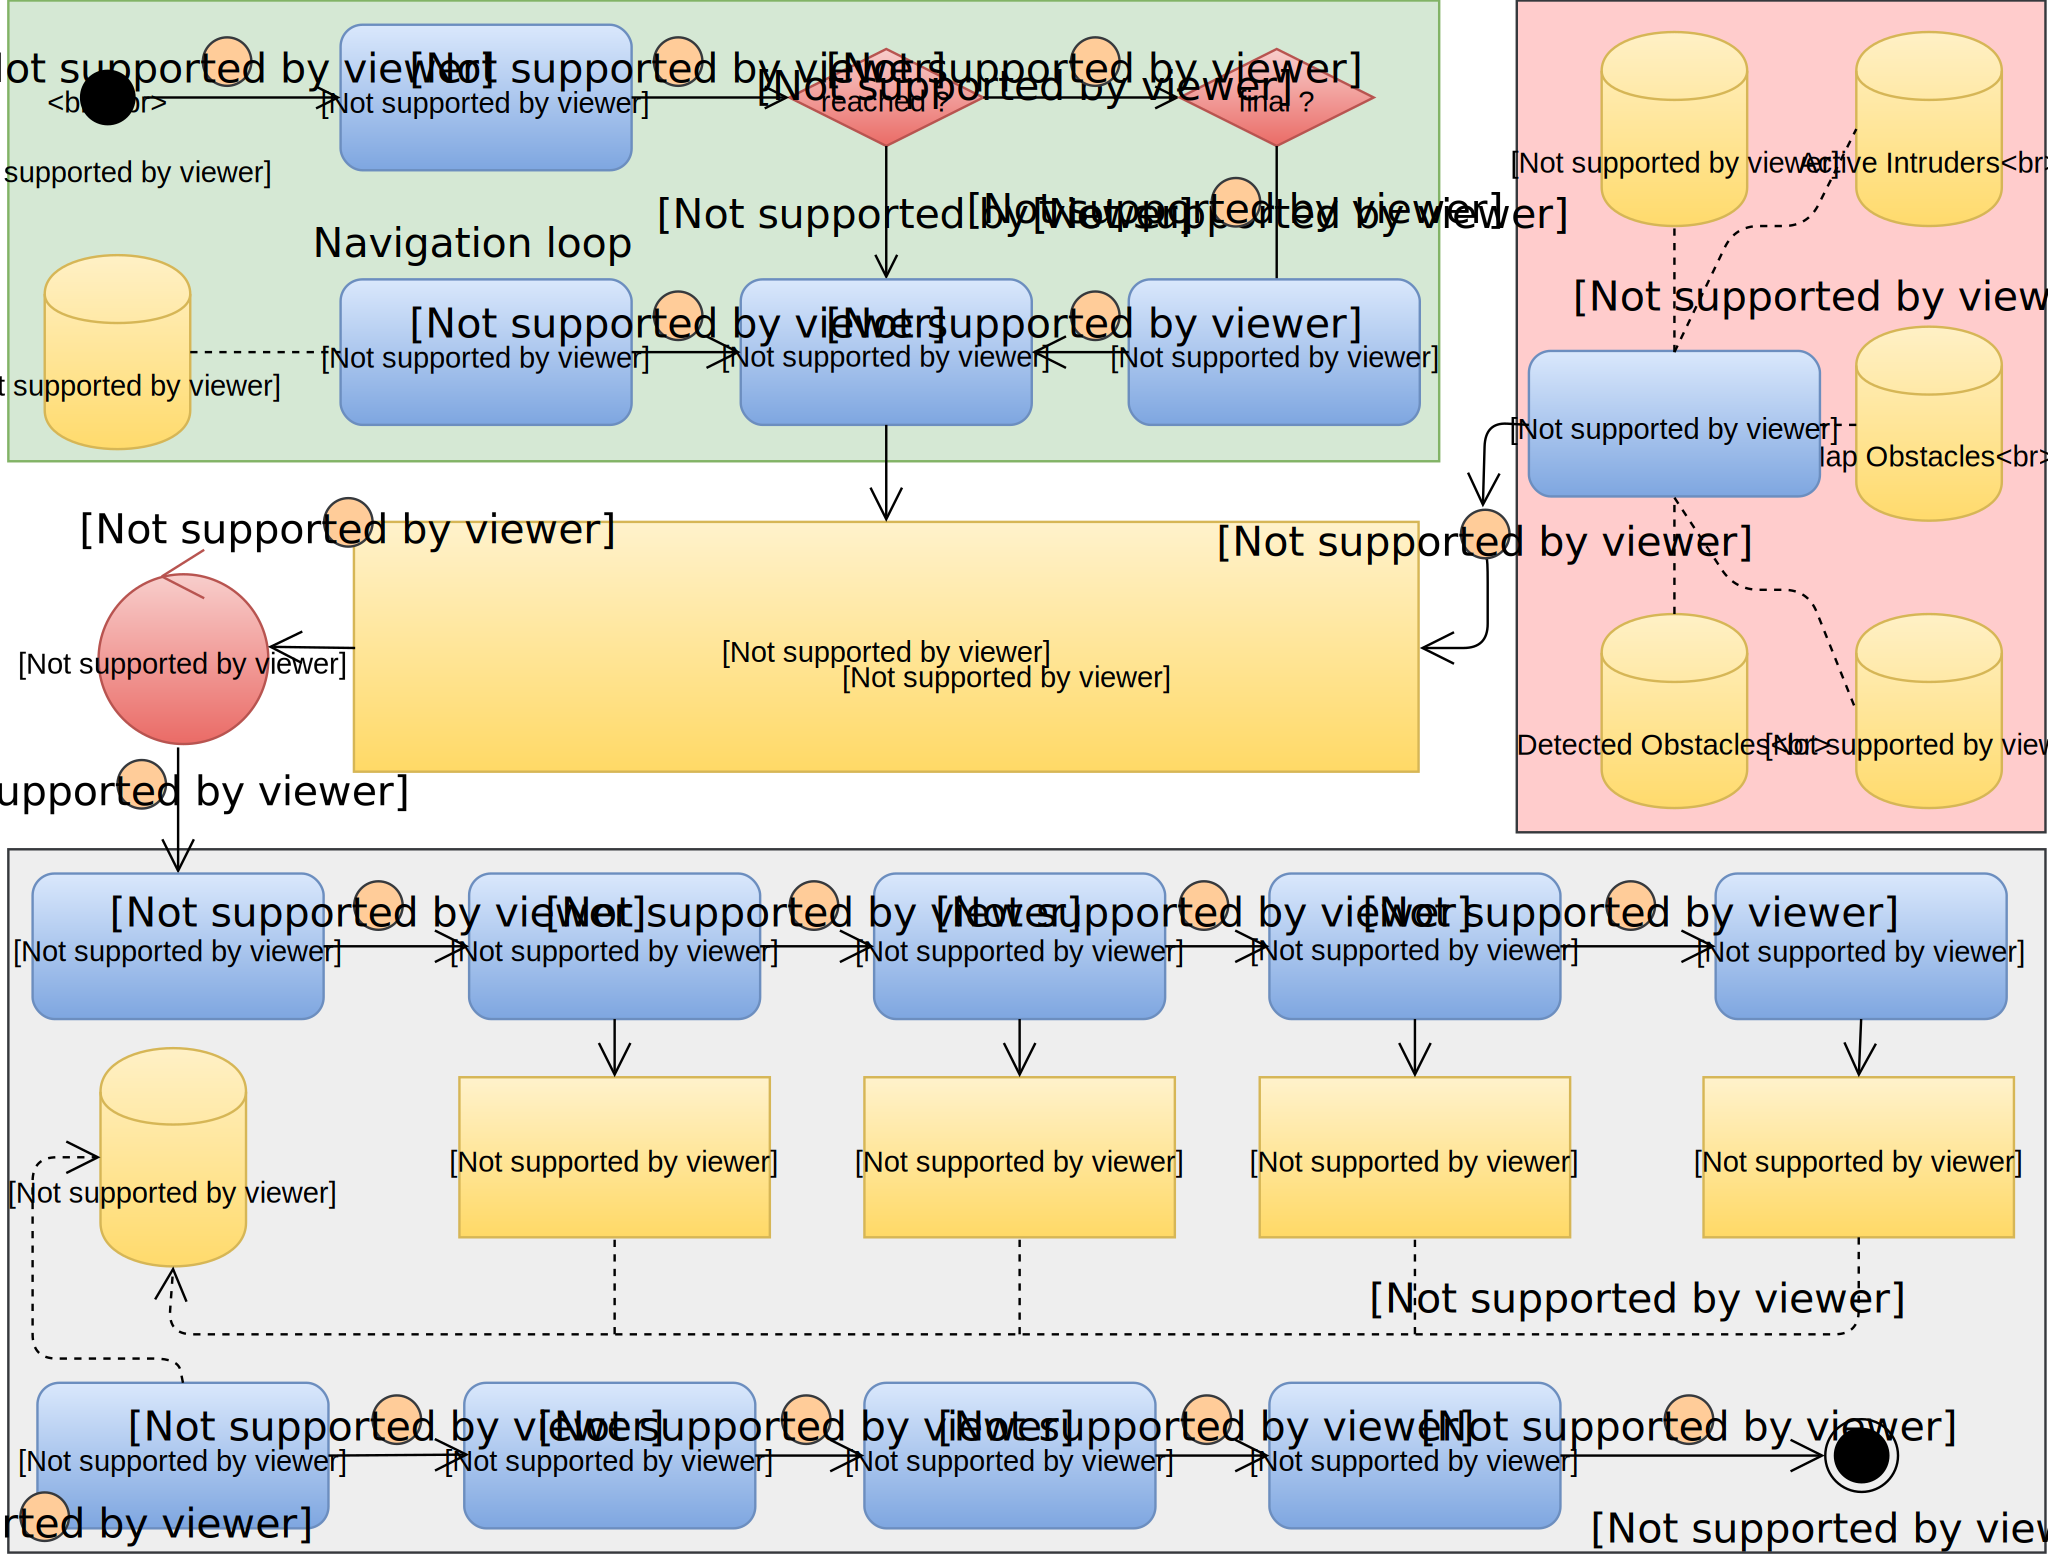
\includegraphics[width=\linewidth]{\FIGDIR/TE026AvoidanceAlgorithmMainLoopRun}
        \caption{Mission control run activity diagram.}
        \label{fig:missionControlRunActivityDiagram}
    \end{figure}

\subsection{(W) Safety margin calculation}\label{s:safetyMarginCalculation}
    How to assess safety margin and what impacts it:
    \begin{itemize}
        \item Own uncertainity 
        \item Intruder uncertainity 
        \item Weather
        \item Airspace
        \item UTM corrections
    \end{itemize}
    
    Note \emph{Both UAS} decision times were \emph{synchronized}, this is not an assumption, but it shows critical performance. Usually safety margin is bloated for:
            \begin{equation}\label{safetyMarginBloat}
                safetyMarginBloat = \left( \begin{aligned}
                &intruderVelocity \times\dots \\ &intruderDecisionFrame \end{aligned}\right)[m,ms^{-1},s]
            \end{equation}
